\documentclass[12pt,letterpaper]{article}
\setcounter{page}{0}

% Figure panel header font
\newcommand{\panel}{\fontfamily{phv}\selectfont\scriptsize\textbf}

% include standard package
\usepackage[latin1]{inputenc}
\usepackage[table]{xcolor}
\usepackage{graphicx}
\usepackage{setspace}
\usepackage{amsmath}
\usepackage{amsthm}
\usepackage{amsfonts}
\usepackage{longtable}
\addtolength{\textwidth}{5cm}
\addtolength{\textheight}{5cm}
\usepackage{fullpage}
\usepackage{amssymb}
\usepackage[hyperpageref]{backref}
\usepackage[hidelinks]{hyperref}
\usepackage{url}
\usepackage{epstopdf}
\usepackage{multirow}
\usepackage{bbm}
\usepackage{tabularx}
\usepackage{floatpag,amsmath,amsthm,amssymb}
\usepackage{float}
\usepackage{lscape}
\usepackage{verbatim}
\usepackage{pdflscape}
\usepackage{chngcntr}
\usepackage{appendix}
\usepackage{booktabs,calc}
\usepackage{ulem}
\usepackage{siunitx}
\usepackage{mathtools}
\usepackage[multiple]{footmisc}

\usepackage{fancyhdr} 
\pagestyle{fancy}
\lhead{}
\chead{}
\rhead{\thepage}
\cfoot{} % get rid of the page number 
\renewcommand{\headrulewidth}{0pt}
\renewcommand{\footrulewidth}{0pt}
\setlength{\headsep}{24pt}

% allow yellow highlighting in tables
\usepackage{color,colortbl}
\usepackage{soul}
\definecolor{Yellow}{rgb}{.88,1,.65}
\definecolor{Green}{rgb}{.65,1,.65}
\definecolor{Red}{rgb}{1,.65,.65}

%\citationstyle{dcu}

\usepackage[labelfont=bf,center,small,labelsep=newline]{caption}
%\usepackage{subfigure}
% \counterwithout{subtable}{table}
\def\changemargin#1#2{\list{}{\rightmargin#2\leftmargin#1}\item[]}
\let\endchangemargin=\endlist

% define subscript / superscript commands
\newcommand{\superscript}[1]{\ensuremath{^{\textrm{#1}}}}
\newcommand{\subscript}[1]{\ensuremath{_{\textrm{#1}}}}

%format paper to save trees
\usepackage[right=1in,left=1in,top=1in,bottom=1in]{geometry}
\usepackage{savetrees}

%AER style headers
\def\thesection{\arabic{section}}
\def\thesubsection {\thesection.\arabic{subsection}}

% set home path
% \newcommand{\HOME}{\string~}

\newcommand{\subfigimg}[3][,]{%
  \setbox1=\hbox{\includegraphics[#1]{#3}}% Store image in box
  \leavevmode\rlap{\usebox1}% Print image
  \rlap{\hspace*{90pt}\raisebox{\dimexpr\ht1+0.9\baselineskip}{\colorbox{white}{{\footnotesize#2}}}}% Print label
  \phantom{\usebox1}% Insert appropriate spcing
}


% SET FILEPATH TO OUTPUTS FOLDER %
\newcommand{\outpath}{\string~/ddl/paper-covid-comorbidities/outputs}

\title{COVID-19 mortality effects of underlying health conditions in
  India: a modelling study: Figures and Tables} \author{Paul Novosad,
  Radhika Jain, Alison Campion, Sam Asher}

%%%%%%%%%%%%%%%%%%%%%% 
% NO TITLE PAGE
%%%%%%%%%%%%%%%%%%%%%% 
\begin{document}
\date{\today}
\maketitle
\clearpage

\begin{figure}
  \begin{center}
    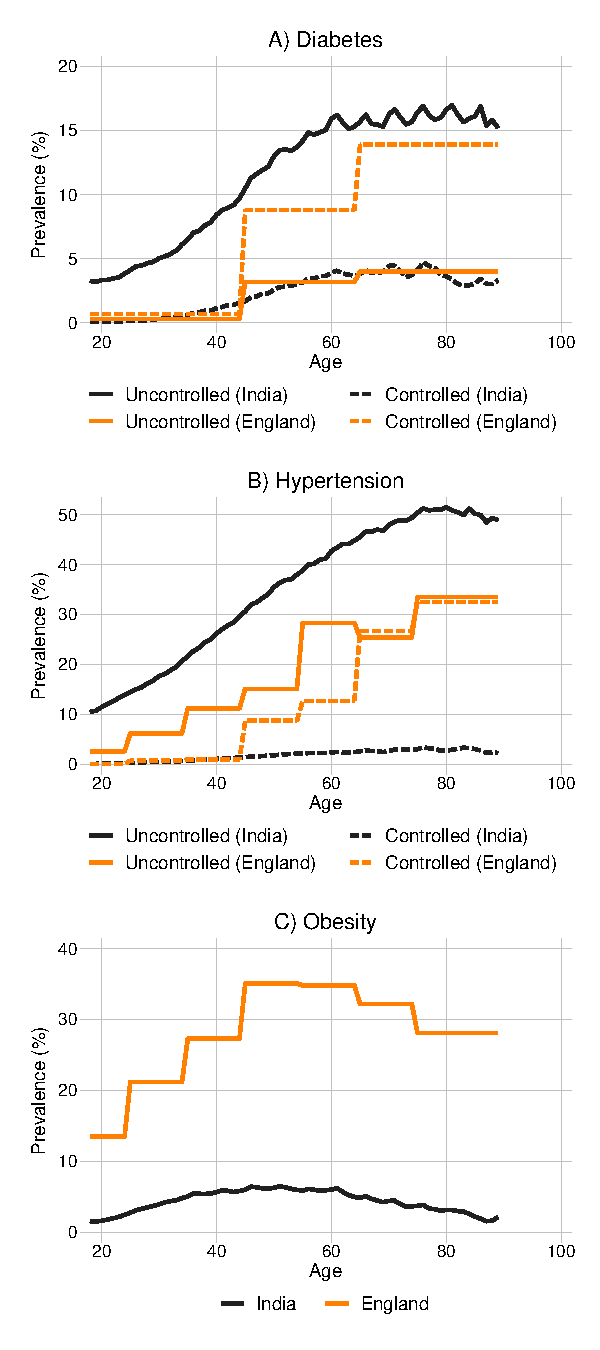
\includegraphics[scale=0.9]{\outpath/three_prevalences.pdf}
  \end{center}
  \caption{Prevalence of (A) diabetes, (B) hypertension, and (C)
    obesity in India and England.}
\end{figure}

\clearpage

\begin{figure}[H]
  \begin{center}
    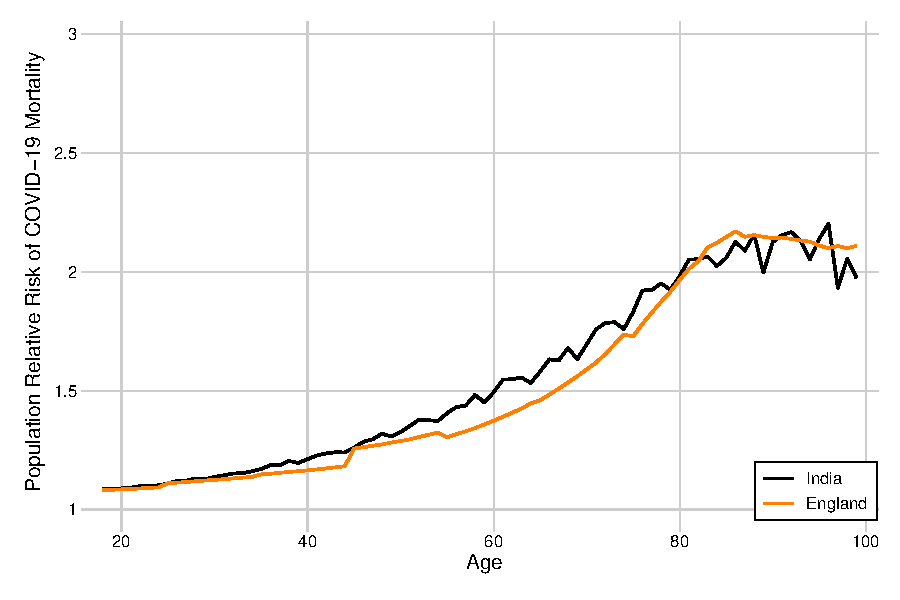
\includegraphics[scale=1.0]{\outpath/prr_health.pdf}
  \end{center}
  \caption{Age-specific population relative risk of COVID-19 mortality from all health conditions ($PRR_{a}$).}
\end{figure}

\begin{figure}[H]
  \begin{center}
    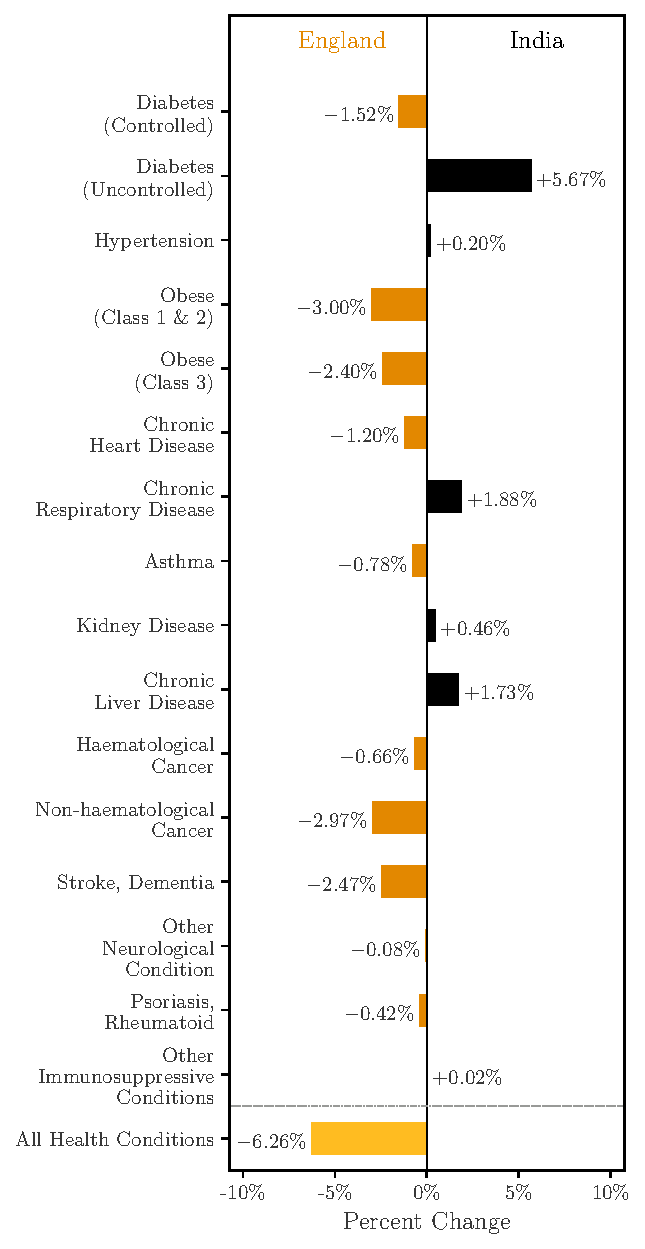
\includegraphics[scale=0.9]{\outpath/coefplot.pdf}
  \end{center}
  \caption{Percent change in population relative risk of COVID-19 mortality from each health condition ($PRR_{c}$) in India versus England.}
\end{figure}

\begin{figure}[H]
  \begin{center}
    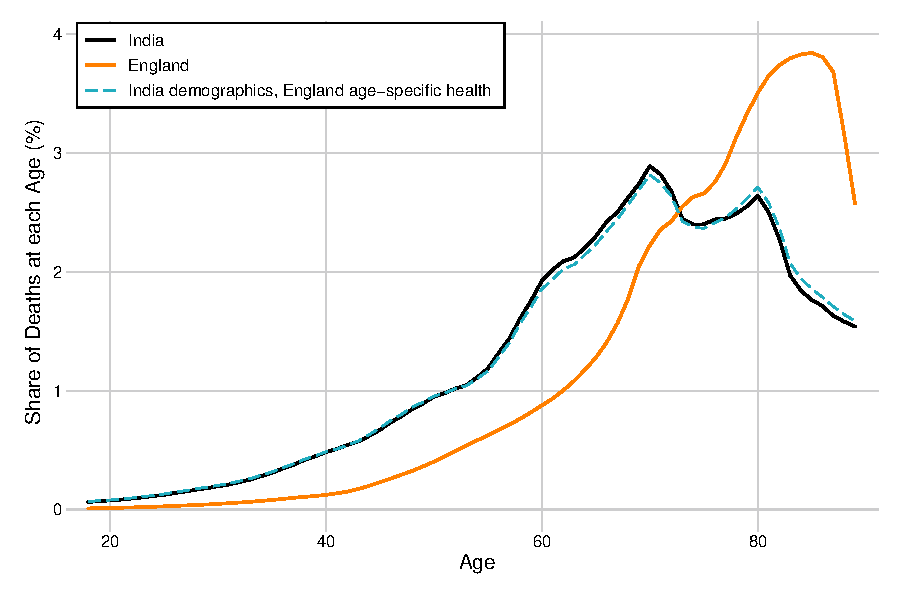
\includegraphics[scale=1.0]{\outpath/mort_density_full.pdf}
  \end{center}
  \caption{Modelled age distribution of COVID-19 mortality.}
\end{figure}

\begin{table}[H]
  \begin{center}
    \begin{tabular}{p{7cm}p{1.1cm}p{1cm}}
& \multicolumn{2}{c}{\textbf{{\footnotesize Prevalence (\%) }}} \\[0.5ex] & \emph{India} & \emph{England} \\[2ex]
Age 18-39 & \num{50.2} & \num{36.6} \\[0.25ex]
Age 40-49 & \num{19.2} & \num{16.3} \\[0.25ex]
Age 50-59 & \num{14.3} & \num{17.0}\\[0.25ex]
Age 60-69 & \num{10.3} & \num{13.3}\\[0.25ex]
Age 70-79 & \num{4.6} & \num{10.4}\\[0.25ex]
Age 80-99 & \num{1.5} & \num{6.3} \\[0.25ex]
Male & \num{47.1} & \num{48.9} \\[0.25ex]
\\
Diabetes (Controlled) & \num{1.7} & \num{6.4} \\[0.25ex]
Diabetes (Uncontrolled) & \num{8.9} & \num{2.1} \\[0.25ex]
Hypertension & \num{28.2} & \num{28.0} \\[0.25ex]
Obese (class I \& II) & \num{4.0} & \num{24.8} \\[0.25ex]
Obese (class III) & \num{0.4} & \num{3.1} \\[0.25ex]
\\
Chronic Heart Disease & \num{4.4} & \num{5.9} \\[0.25ex]
Chronic Respiratory Disease & \num{4.8} & \num{2.5} \\[0.25ex]
Asthma & \num{2.5} & \num{9.2} \\[0.25ex]
Kidney Disease & \num{9.7} & \num{5.6} \\[0.25ex]
Chronic Liver Disease & \num{5.3} & \num{2.6} \\[0.25ex]
\\
Haematological Cancer & \num{0.0} & \num{0.2}\\[0.25ex]
Non-haematological Cancer & \num{0.3} & \num{2.6} \\[0.25ex]
Stroke, Dementia & \num{1.3} & \num{1.5} \\[0.25ex]
Other Neurological Condition & \num{0.0} & \num{0.1} \\[0.25ex]
Psoriasis, Rheumatoid & \num{1.0} & \num{2.4} \\[0.25ex]
Other Immunosuppressive Conditions & \num{0.1} & \num{0.1} \\[0.25ex]
\end{tabular}

  \end{center}
  \caption{Prevalence of COVID-19 risk factors in India and England.}  
\end{table}

\begin{table}[H]
  \begin{center}
    \begin{tabular}{p{7cm}cp{1.25cm}p{1.5cm}}
& \textbf{{\footnotesize Individual}} &
  \multicolumn{2}{c}{{\textbf{\footnotesize{Population}}}} \\
& \textbf{{\footnotesize Relative Risk}} &
  \multicolumn{2}{c}{{\textbf{\footnotesize{Relative Risk}}}} \\[0.75ex]
  & & \emph{India} & \emph{England} \\[2ex]
%Male & 1.99 & \num{1.298} & \num{1.286} \\[0.25ex]
Diabetes (Controlled) & \num{1.31} & \num{1.004} & \num{1.020} \\[0.25ex]
Diabetes (Uncontrolled) & \num{1.94} & \num{1.078} & \num{1.020} \\[0.25ex]
Hypertension & \num{0.89} & \num{0.971} & \num{0.969} \\[0.25ex]
Obese (class I \& II) & \num{1.15} & \num{1.006} & \num{1.037} \\[0.25ex]
Obese (class III) & \num{1.91} & \num{1.004} & \num{1.028} \\[0.25ex]
\\
Chronic Heart Disease & \num{1.17} & \num{1.008} & \num{1.021} \\[0.25ex]
Chronic Respiratory Disease & \num{1.62} & \num{1.035} & \num{1.015} \\[0.25ex]
Asthma & \num{1.13} & \num{1.003} & \num{1.011} \\[0.25ex]
Kidney Disease & \num{1.42} & \num{1.050} & \num{1.046} \\[0.25ex]
Chronic Liver Disease & \num{1.73} & \num{1.042} & \num{1.024} \\[0.25ex]
\\
Haematological Cancer & \num{2.79} & \num{1.000} & \num{1.007} \\[0.25ex]
Non-haematological Cancer & \num{1.71} & \num{1.003} & \num{1.033} \\[0.25ex]
Stroke, Dementia & \num{2.15} & \num{1.016} & \num{1.041} \\[0.25ex]
Other Neurological Condition & \num{2.56} & \num{1.002} & \num{1.002} \\[0.25ex]
Psoriasis, Rheumatoid & \num{1.19} & \num{1.002} & \num{1.007} \\[0.25ex]
Other Immunosuppressive Conditions & \num{1.69} & \num{1.001} & \num{1.001} \\[0.25ex]
\end{tabular}


  \end{center}
  \caption{Population relative risk of COVID-19 mortality from each health condition ($PRR_{c}$)}
\end{table}


\end{document}

